\documentclass{article}
\usepackage{graphicx}
\usepackage{fancyhdr}
\usepackage{listings}

\let\<\textless
\let\>\textgreater

\graphicspath{ {images/} }
\pagestyle{fancy}
\fancyhf{}
\rhead{Proyecto \#2}
\rfoot{P\'agina \thepage}

\begin{document}
\begin{titlepage}
  \centering
  {\scshape\LARGE Instituto Tecnol\'ogico de Costa Rica \par}
  \vspace{1cm}
  {\scshape\Large Proyecto \#2\par}
  \vspace{1.5cm}
  {\Large\itshape Alejandro Rojas\par}
  {\Large\itshape Sa\'ul Zamora\par}
  \vfill
  profesor\par
  Kevin Moraga \textsc{}

  \vfill

% Bottom of the page
  {\large \today\par}
\end{titlepage}

\section{Introducci\'on}
Se requiere un sistema para una empresa productora de dispositivos de IoT (Internet Of Things), los cuales se distribuyen a nivel nacional y se exporta a Nicaragua, Panam\'a y Guatemala.

Uno de los principales negocios de la empresa son las ``Smart Houses'', lo cual implica brindarle al cliente una experiencia \'unica al darle control total de su casa y los dispositivos en ella.

Las bases de datos deben almacenar informaci\'on de forma local y otros datos de forma remota en las instalaciones de la empresa. Actualmente, las tecnolog\'ias usadas son MySQL, SQL Server y Oracle.

La base de datos de producci\'on posee un inventario de todas las partes que la empresa adquiere como materia prima para la creaci\'on de los dispositivos. Existe otro sistema que usa otra base de datos donde se controlan las ventas de los productos y dispositivos, la cual es b\'asicamente un cat\'alogo de los productos; adem\'as de un historial con los cambios en los precios de dichos productos.

Cada casa de habitaci\'on cuenta con una base de datos local, cuya funci\'on principal es recolectar informaci\'on post-venta de los dispositivos e informaci\'on generada por su uso.

Es requerido mantener las bases de datos locales y remotas replicadas para brindarle al usuario la experiencia que desea.

Adem\'as, el sistema deseado debe ser capaz de producir estad\'isticas sobre inteligencia de negocios con el fin de ayudar a la gerencia a tomar decisiones m\'as acertadas. Algunos de los puntos m\'as relevantes son:

\begin{itemize}
  \item Costos de producci\'on
  \item Sugerencias de consumo de productos del cliente en los pr\'oximos 15 d\'ias.
  \item Dispositivos IoT m\'as utilizados por un cliente
  \item Dispositivos IoT m\'as vendidos
  \item Tiempo de entrega de materiales relacionados a los dispositivos IoT m\'as vendidos
  \item Estad\'isticas sobre los proveedores (calidad de materiales, precios, etc)
  \item Determinar los materiales de mayor y menor circulaci\'on
  \item Estad\'isticas sobre las ventas anuales
  \item Estad\'isticas sobre los carriers de los productos (volumen enviado, m\'as utilizados, destinos, etc)
  \item \'Indices de ganancias vs \'indices de gastos
\end{itemize}

\section{Ambiente de desarrollo}
\begin{itemize}
  \item Sistema operativo host utilizado: Windows 10
  \item Python 3.6 (Simulaci\'on)
  \item Oracle VirtualBox 5.1
  \item Windows Server 2008 R2 (Dos m\'aquinas virtuales)
  \item SQL Server 2008 Enterprise
  \item Pentaho 7.1
\end{itemize}

\section{Estructuras de datos usadas y funciones}
Para la simulaci\'on se usaron listas para almacenar datos aleatorios, los cuales luego se guardan en archivos CSV. El archivo de simulaci\'on genera todos los datos en una sola corrida, por lo que no utiliza otras funciones en particular. Sin embargo, se utilizaron las siguientes librer\'ias para su correcta ejecuci\'on:
\begin{itemize}
  \item csv
  \item random (randint)
  \item datetime (date, timedelta)
  \item operator
  \item numpy
\end{itemize}

\section{Instrucciones para ejecutar el programa}
Para generar los archivos CSV con los datos simulados, hay que colocar el archivo \emph{dataSimulator.py} en la carpeta que se desea almacenarlos. Loego se debe ejecutar ya sea mediante el IDLE de Python, presionando F5, o mediante la l\'inea de comandos, ejecutando directamente el programa.

Una vez generados los archivos, se puede utilizar el servicio de \emph{import} de SQL Server para insertar los datos en las bases de datos respectivas.

\section{Bit\'acora de trabajo}
\subsection{Alejandro Rojas}
\begin{itemize}
  \item 12-06-2017:
  \begin{itemize}
    \item 1.5 horas - Descarga e instalaci\'on de Pentaho y Windows Server 2008 R2.
  \end{itemize}
  \item 13-06-2017:
  \begin{itemize}
    \item 4 horas - Dise\~no de base de datos y simulaci\'on. Dise\~no y simulaci\'on de productos y distribuidores.
  \end{itemize}
  \item 14-06-2017:
  \begin{itemize}
    \item 8 horas - Dise\~no y simulaci\'on de materiales, categor\'ias, modelos, etc.
  \end{itemize}
  \item 15-06-2017:
  \begin{itemize}
    \item 5 horas - Simulaci\'on de ventas y despachos de productos.
  \end{itemize}
  \item 17-06-2017:
  \begin{itemize}
    \item 4 horas - Detalles de la simulaci\'on.
  \end{itemize}
  \item 18-06-2017:
  \begin{itemize}
    \item 3 horas - Conectar 2 m\'aquinas virtuales con Windows Server 2008 R2.
    \item 2 horas - Crear carpetas compartidas para archivos CSV, Excel y Replicaciones. Configuraci\'on correcta de la replicaci\'on de la base de datos de inventorio en la segunda m\'aquina virtual.
    \item 1.5 horas - Configuraci\'on correcta de la replicaci\'on de la base de datos de ventas en la primera m\'aquina virtual.
    \item 1 hora - Terminar llenado de la base de datos de inventarios.
  \end{itemize}
  \item 19-06-2016:
  \begin{itemize}
    \item 8 horas - Configuraci\'on de Pentaho y proceso de ETL / reportes.
  \end{itemize}
  \item Total horas: 38 horas.
\end{itemize}

\subsection{Sa\'ul Zamora}
\begin{itemize}
  \item 12-06-2017:
  \begin{itemize}
    \item 2 horas - Investigaci\'on sobre replicaci\'on de base de datos en SQL Server 2008 Enterprise.
  \end{itemize}
  \item 13-06-2017:
  \begin{itemize}
    \item 5 horas - Descarga de Windows Server 2008 R2 y configuraci\'on de la primera m\'aquina virtual.
  \end{itemize}
  \item 14-06-2017:
  \begin{itemize}
    \item 1 hora - Configuraci\'on de la segunda m\'aquina virtual con Windows Server 2008 R2.
    \item 3 horas - Descarga de SQL Server Enterprise.
  \end{itemize}
  \item 15-06-2017:
  \begin{itemize}
    \item 2 horas - Instalaci\'on de SQL Server en ambas m\'aquinas virtuales.
    \item 2 horas - Configuraci\'on de carpetas compartidas en las m\'aquinas virtuales para archivos CSV.
  \end{itemize}
  \item 17-06-2017:
  \begin{itemize}
    \item 5 horas - Intento de configuraci\'on de replicaci\'on de bases de datos con las m\'aquinas virtuales de Windows Server y SQL Server.
  \end{itemize}
  \item 19-06-2017:
  \begin{itemize}
    \item 4 horas - Documentaci\'on.
  \end{itemize}
  \item Total horas: 25 horas.
\end{itemize}

\section{Comentarios finales}

\section{Conclusiones}
\begin{itemize}
  \item Es importante tomar en cuenta la configuraci\'on en el firewall de Windows Server 2008 R2 a la hora de configurar m\'aquinas virtuales con el prop\'osito de que sean capaces de ``verse entre s\'i''.
\end{itemize}

\begin{thebibliography}{99}
\bibitem{replication}  Singh, S. (2017). SQL Server Performance Setting up Transactional Replication in SQL Server 2008 R2. [online] Sql-server-performance.com. Available at: \texttt{http://www.sql-server-performance.com/2010/transactional-replication-2008-r2/}
\end{thebibliography}

\section{Anexos}
\begin{figure}[!ht]
  \caption{Diagrama de la base de datos de Inventario}
  \centering
    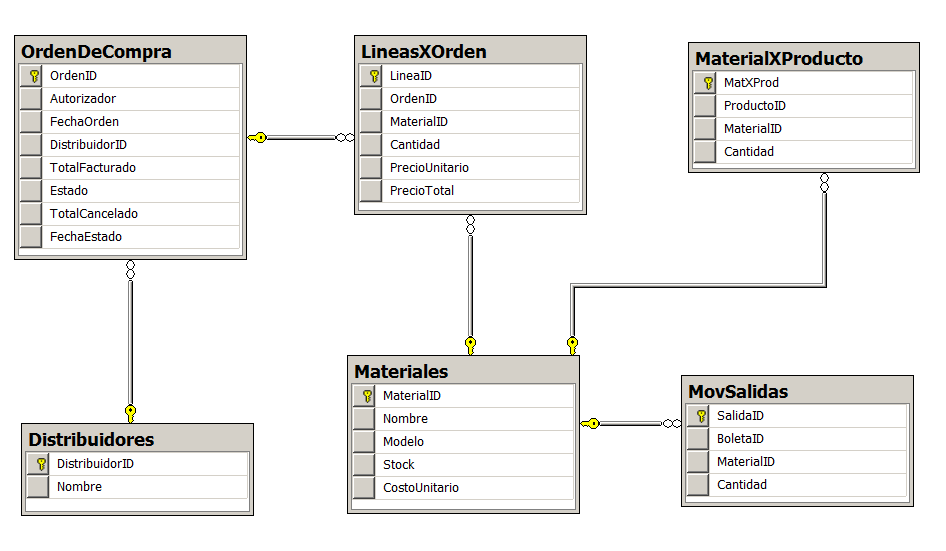
\includegraphics[width=1\textwidth]{diagInv.PNG}
\end{figure}

\begin{figure}[!ht]
  \caption{Diagrama de la base de datos de Ventas}
  \centering
    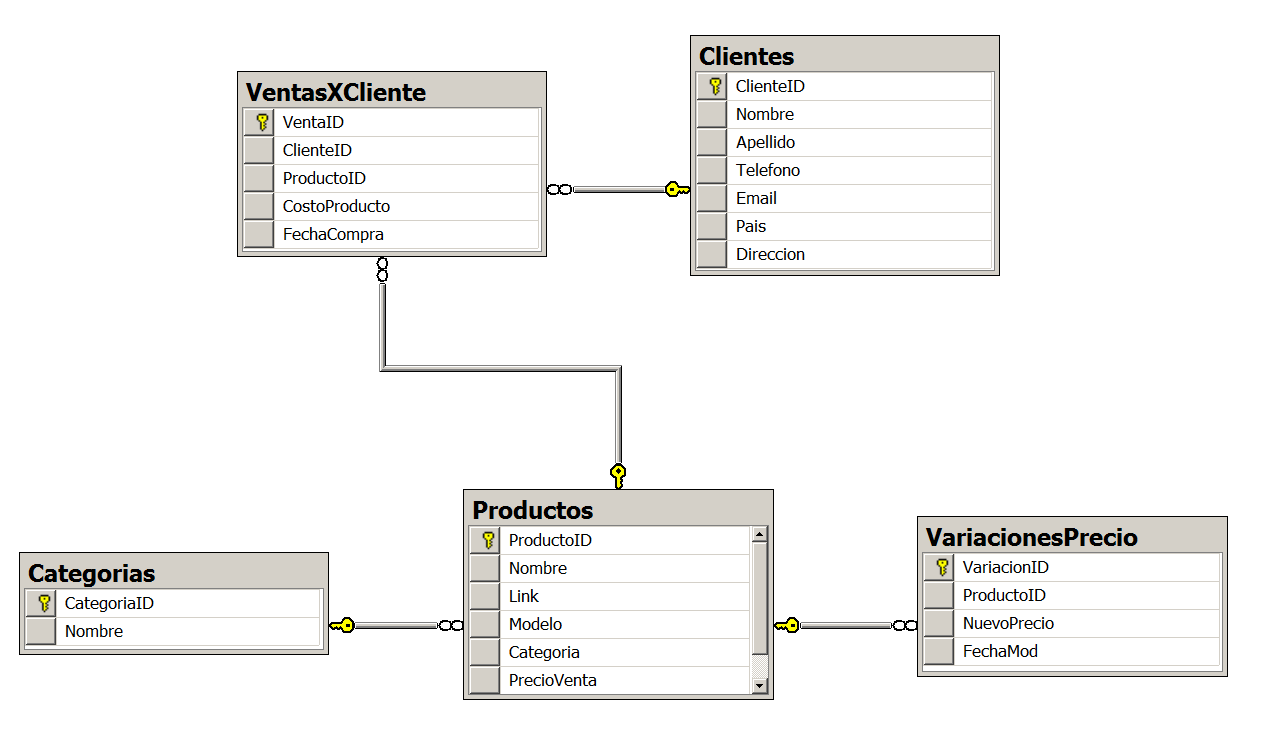
\includegraphics[width=1\textwidth]{diagVentas.PNG}
\end{figure}

\begin{figure}[!ht]
  \caption{Configuraci\'on de conexi\'on a Pentaho}
  \centering
    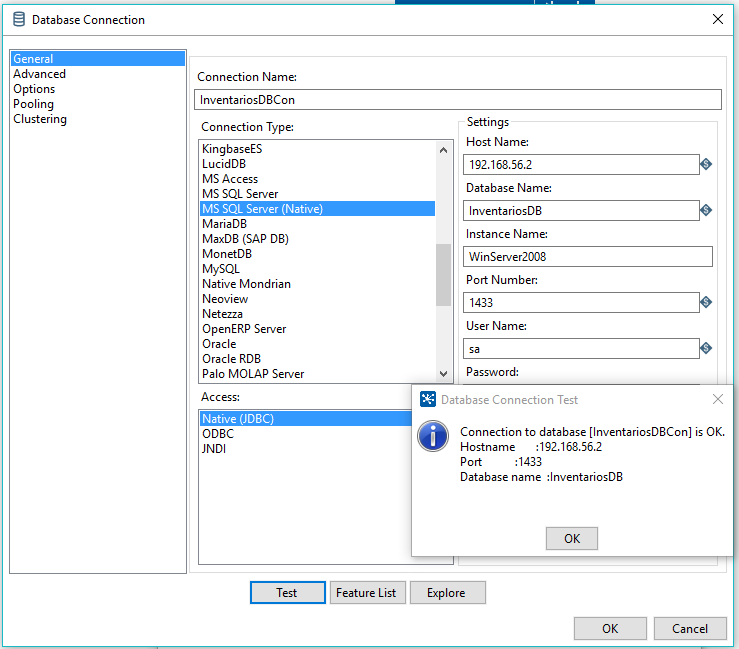
\includegraphics[width=1\textwidth]{pentahoDBCon1.PNG}
\end{figure}

\begin{figure}[!ht]
  \caption{Estados de las bases de datos replicadas}
  \centering
    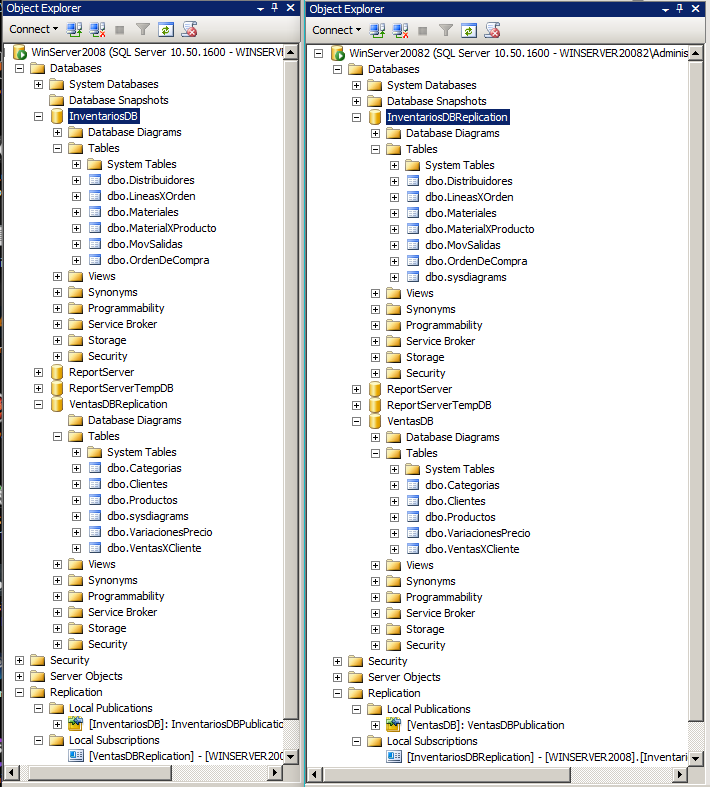
\includegraphics[width=1\textwidth]{replicacionFull.PNG}
\end{figure}

\end{document}